\begin{figure}[p]
\centering
% The Argument plate rendered natively in TikZ so edge attestations are clickable.
\begingroup
\footnotesize
\newcommand{\hash}[1]{\href{https://github.com/tothedarktowercame/futon6/commit/#1}{\texttt{#1}}}
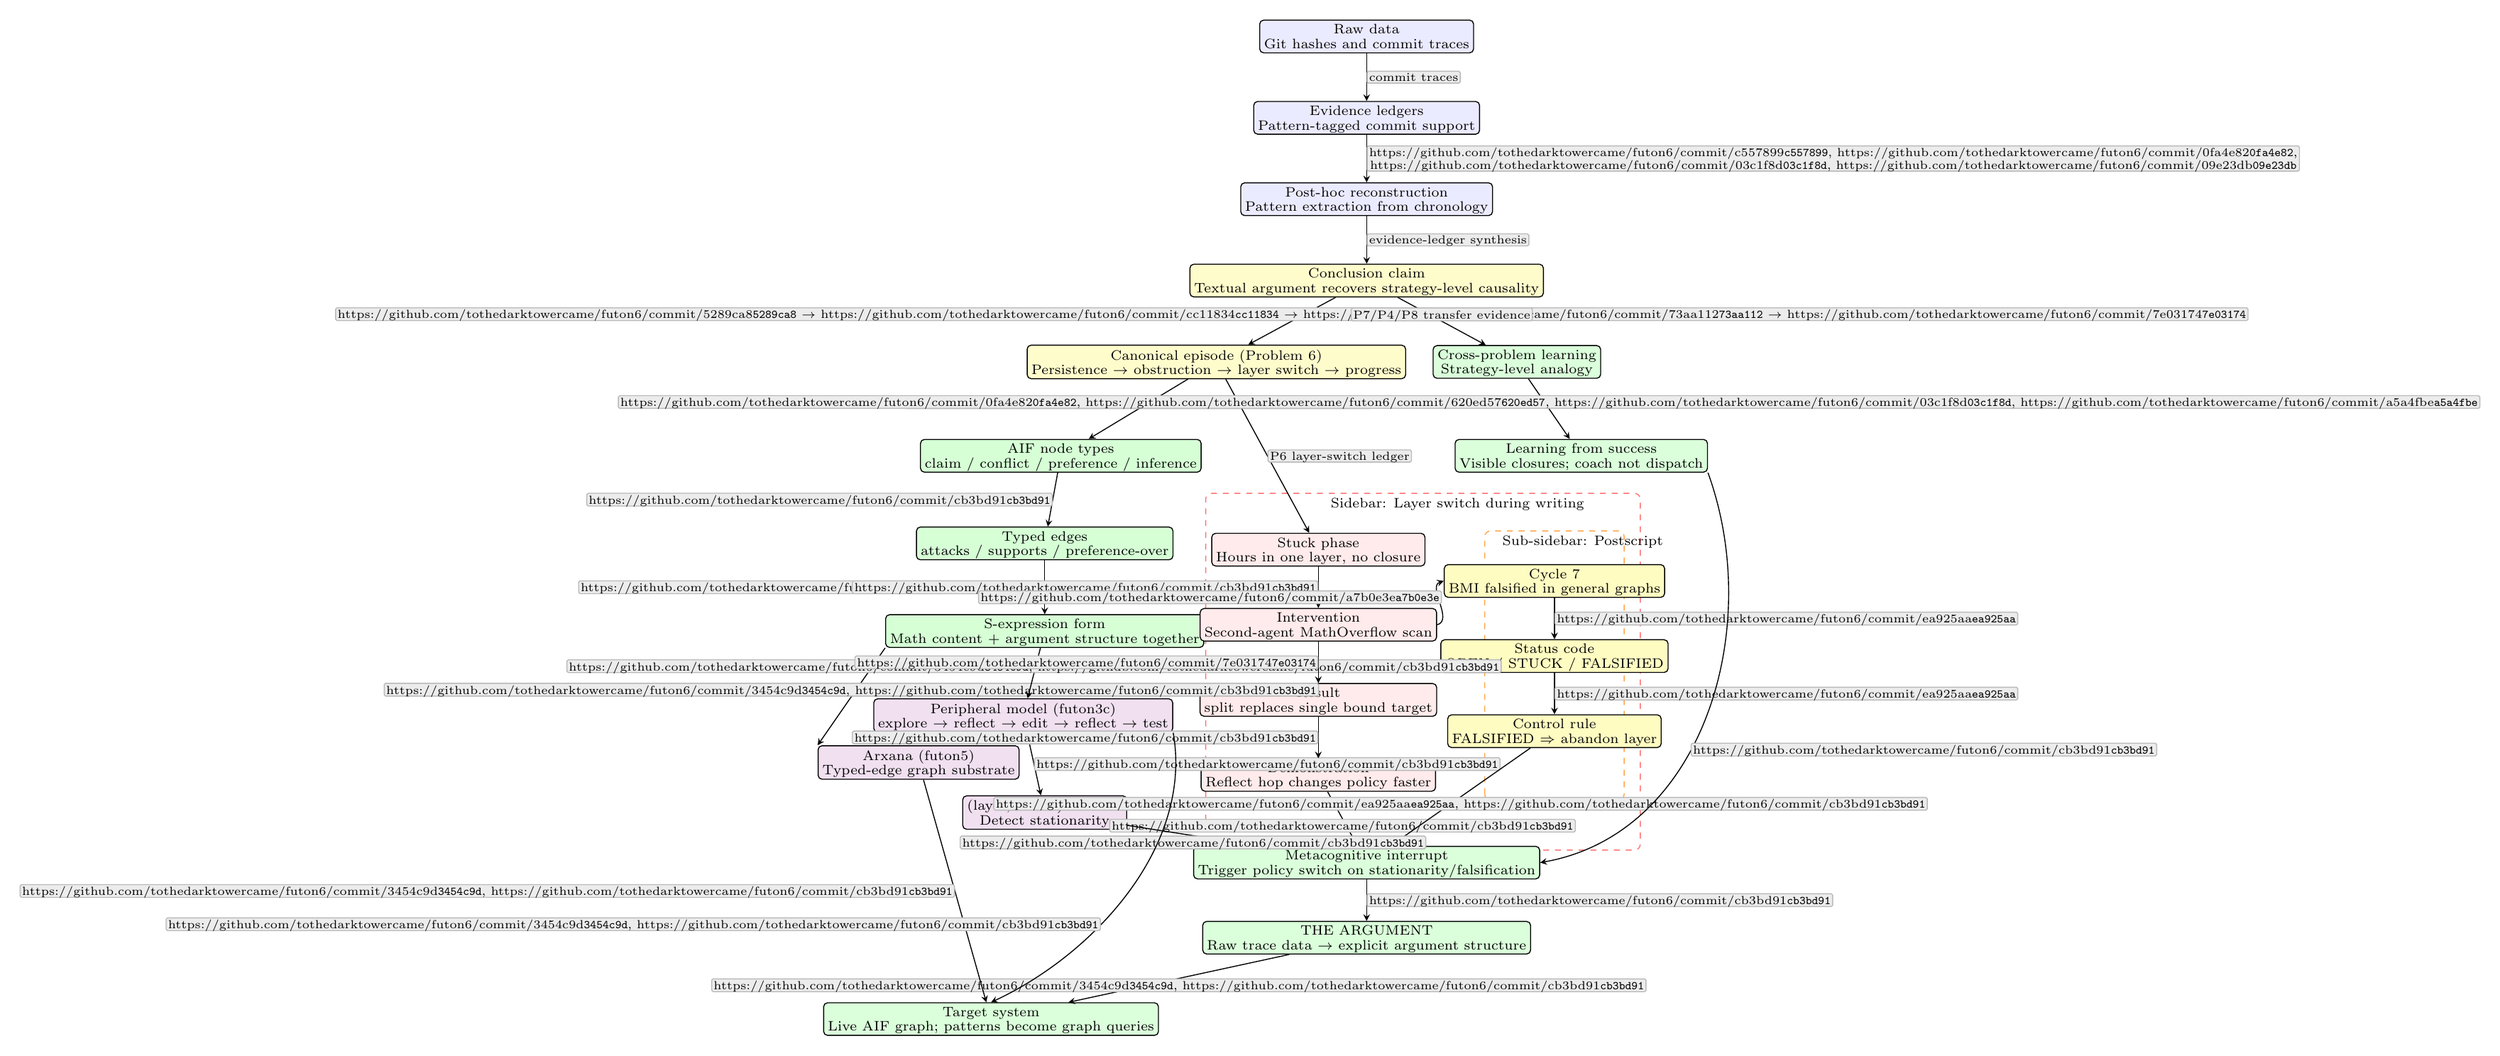
\begin{tikzpicture}[
  x=0.96cm,
  y=1.12cm,
  >=stealth,
  line width=0.5pt,
  text depth=0pt,
  hashlbl/.style={fill=gray!15,draw=gray!55,rounded corners=0.7pt,inner sep=1.0pt,font=\fontsize{5.8}{6.3}\selectfont,align=center},
  box/.style={draw,rounded corners=2pt,align=center,inner sep=2.2pt,font=\fontsize{6.6}{7.4}\selectfont},
  data/.style={box,fill=blue!8},
  synth/.style={box,fill=yellow!20},
  formal/.style={box,fill=green!16},
  infra/.style={box,fill=violet!12},
  side/.style={box,fill=red!8},
  post/.style={box,fill=yellow!24},
  outc/.style={box,fill=green!14}
]

% Top chain
\node[data] (G0) at (0,14.2) {Raw data\\Git hashes and commit traces};
\node[data] (G1) at (0,12.9) {Evidence ledgers\\Pattern-tagged commit support};
\node[data] (G2) at (0,11.6) {Post-hoc reconstruction\\Pattern extraction from chronology};
\node[synth] (C0) at (0,10.3) {Conclusion claim\\Textual argument recovers strategy-level causality};

% Mid layer
\node[synth] (C1) at (-2.8,9.0) {Canonical episode (Problem 6)\\Persistence $\to$ obstruction $\to$ layer switch $\to$ progress};
\node[outc]  (X0) at (2.8,9.0) {Cross-problem learning\\Strategy-level analogy};

% Left formal/infrastructure
\node[formal] (A0) at (-5.7,7.5) {AIF node types\\claim / conflict / preference / inference};
\node[formal] (A1) at (-6.0,6.1) {Typed edges\\attacks / supports / preference-over};
\node[formal] (A2) at (-6.0,4.7) {S-expression form\\Math content + argument structure together};
\node[infra]  (I0) at (-8.35,2.60) {Arxana (futon5)\\Typed-edge graph substrate};
\node[infra]  (I1) at (-6.4,3.35) {Peripheral model (futon3c)\\explore $\to$ reflect $\to$ edit $\to$ reflect $\to$ test};
\node[infra]  (I2) at (-6.0,1.8) {(layer, status) monitor\\Detect stationarity};

% Right learning
\node[outc] (X1) at (4.0,7.5) {Learning from success\\Visible closures; coach not dispatch};

% Sidebar region
\draw[red!55,dashed,rounded corners=3pt] (-3.0,1.2) rectangle (5.1,6.9);
\node[font=\scriptsize,anchor=west] at (-0.8,6.75) {Sidebar: Layer switch during writing};

\node[side] (S0) at (-0.9,6.0) {Stuck phase\\Hours in one layer, no closure};
\node[side] (S1) at (-0.9,4.8) {Intervention\\Second-agent MathOverflow scan};
\node[side] (S2) at (-0.9,3.6) {Result\\split replaces single bound target};
\node[side] (S3) at (-0.9,2.4) {Demonstration\\Reflect hop changes policy faster};

\draw[orange!70,dashed,rounded corners=3pt] (2.2,2.0) rectangle (4.8,6.3);
\node[font=\scriptsize,anchor=west] at (2.4,6.15) {Sub-sidebar: Postscript};
\node[post] (P0) at (3.5,5.5) {Cycle 7\\BMI falsified in general graphs};
\node[post] (P1) at (3.5,4.3) {Status code\\OPEN / STUCK / FALSIFIED};
\node[post] (P2) at (3.5,3.1) {Control rule\\FALSIFIED $\Rightarrow$ abandon layer};

% Bottom
\node[outc] (X2) at (0.0,1.0) {Metacognitive interrupt\\Trigger policy switch on stationarity/falsification};
\node[outc] (T0) at (0.0,-0.2) {THE ARGUMENT\\Raw trace data $\to$ explicit argument structure};
\node[outc] (T1) at (-7.0,-1.5) {Target system\\Live AIF graph; patterns become graph queries};

% Edges and labels
\draw[->] (G0) -- (G1) node[midway,right,hashlbl] {commit traces};
\draw[->] (G1) -- (G2) node[midway,right,hashlbl] {\hash{c557899}, \hash{0fa4e82},\\\hash{03c1f8d}, \hash{09e23db}};
\draw[->] (G2) -- (C0) node[midway,right,hashlbl] {evidence-ledger synthesis};
\draw[->] (C0) -- (C1) node[midway,above,hashlbl] {\hash{5289ca8} $\to$ \hash{cc11834} $\to$ \hash{73aa112} $\to$ \hash{7e03174}};
\draw[->] (C0) -- (X0) node[midway,above,hashlbl] {P7/P4/P8 transfer evidence};

\draw[->] (C1) -- (A0) node[midway,above,hashlbl] {\hash{cb3bd91}};
\draw[->] (A0) -- (A1) node[midway,left,hashlbl] {\hash{cb3bd91}};
\draw[->] (A1) -- (A2) node[midway,left,hashlbl] {\hash{cb3bd91}};
\draw[->] (A2.south west) -- (I0.north west) node[midway,above,hashlbl] {\hash{3454c9d}, \hash{cb3bd91}};
\draw[->] (A2) -- (I1) node[midway,above,hashlbl] {\hash{3454c9d}, \hash{cb3bd91}};
\draw[->] (I1) -- (I2) node[midway,right,hashlbl] {\hash{cb3bd91}};

\draw[->] (C1) -- (S0) node[midway,right,hashlbl] {P6 layer-switch ledger};
\draw[->] (S0) -- (S1) node[midway,left,hashlbl] {\hash{cb3bd91}};
\draw[->] (S1) -- (S2) node[midway,left,hashlbl] {\hash{7e03174}};
\draw[->] (S1.east) to[out=14,in=198] node[pos=0.40,left,yshift=6pt,hashlbl] {\hash{a7b0e3e}} (P0.west);
\draw[->] (S2) -- (S3) node[midway,left,hashlbl] {\hash{cb3bd91}};
\draw[->] (S3) -- (X2) node[midway,below,hashlbl] {\hash{cb3bd91}};

\draw[->] (P0) -- (P1) node[midway,right,hashlbl] {\hash{ea925aa}};
\draw[->] (P1) -- (P2) node[midway,right,hashlbl] {\hash{ea925aa}};
\draw[->] (P2) -- (X2) node[midway,below,hashlbl] {\hash{ea925aa}, \hash{cb3bd91}};

\draw[->] (X0) -- (X1) node[midway,above,hashlbl] {\hash{0fa4e82}, \hash{620ed57}, \hash{03c1f8d}, \hash{a5a4fbe}};
\draw[->] (X1.south east) to[out=-70,in=10] node[pos=0.58,right,hashlbl] {\hash{cb3bd91}} (X2.east);
\draw[->] (I2) -- (X2) node[midway,below,hashlbl] {\hash{cb3bd91}};
\draw[->] (X2) -- (T0) node[midway,right,hashlbl] {\hash{cb3bd91}};
\draw[->] (T0) -- (T1) node[midway,below,hashlbl] {\hash{3454c9d}, \hash{cb3bd91}};
\draw[->] (I0) -- (T1) node[midway,left,hashlbl] {\hash{3454c9d}, \hash{cb3bd91}};
\draw[->] (I1.south east) to[out=-80,in=25,looseness=0.90] node[pos=0.62,left,hashlbl] {\hash{3454c9d}, \hash{cb3bd91}} (T1.north);

\end{tikzpicture}
\endgroup

\caption{The Argument (Conclusion recapitulation): git hashes as raw trace data feed evidence ledgers and post-hoc pattern reconstruction; the conclusion makes this into an explicit argument (AIF node/edge typing, S-expression form, and infrastructure path via Arxana plus peripherals). The sidebar and sub-sidebar episodes are integrated as live evidence for the metacognitive interrupt claim: monitor \((\mathrm{layer},\mathrm{status})\), trigger policy switch on stationarity/falsification, and move from retrospective prose toward real-time argumentative structure.}
\end{figure}
\clearpage

\begin{figure}[p]
\centering
\includegraphics[width=\textwidth,height=0.86\textheight,keepaspectratio]{plates/problem6-a-to-ef-v2.png}
\caption{Problem 6 strategy flow (v2, 9-cycle): from leverage-split dispatch through Neumann/operator-bound attack (C4), BR1--BR4 blocking and threshold relaxation (C5), bridge~B leverage-ordered greedy (C6), BMI falsification (C7), to the Sparse/Strong Dichotomy resolution (C9). Green = proved, yellow = pivot/open, dashed red = falsified. $K_n$ closed with $c_0 = 1/3$; general case conditional on the Strong Dichotomy conjecture (0/148 counterexamples).}
\end{figure}
\clearpage

\begin{figure}[p]
\centering
\includegraphics[width=\textwidth,height=0.86\textheight,keepaspectratio]{plates/problem6-v6.png}
\caption{Problem 6 strategy flow (v6, Cycle~4 focus): operator-bound reduction around the Tur\'an/greedy/pigeonhole core, with Neumann-series amplification controlled via monotonicity and an operator bound for \(\rho_1\). Remaining open node: the trace-gap inequality (\(\alpha < 1/2\), equivalently \(\mathrm{tr}(F) > 2\sum \mu_i(1-\mu_i)/\mu_{\max}\)) needed for full general-graph closure.}
\end{figure}
\clearpage

\begin{figure}[p]
\centering
\includegraphics[angle=90,totalheight=0.86\textheight,keepaspectratio]{plates/problem4-v3.png}
\caption{Problem 4 (v3): finite-free Stam architecture with case decomposition and proof-status stratification.}
\end{figure}
\clearpage

\begin{figure}[p]
\centering
\includegraphics[width=\textwidth,height=0.86\textheight,keepaspectratio]{plates/problem8-v3.png}
\caption{Problem 8 (v3): Lagrangian polyhedral smoothing route with product-smoothing and edge generating-function steps.}
\end{figure}
\clearpage

\begin{figure}[p]
\centering
\includegraphics[width=\textwidth,height=0.86\textheight,keepaspectratio]{plates/problem9-v2.png}
\caption{Problem 9 (v2): rank-1 scaling characterization and polynomial nonvanishing witness flow.}
\end{figure}
\clearpage

\begin{figure}[p]
\centering
\includegraphics[width=\textwidth,height=0.86\textheight,keepaspectratio]{plates/problem10-v2.png}
\caption{Problem 10 (v2): preconditioned-Kronecker solve architecture and complexity path.}
\end{figure}
\clearpage
